\documentclass{beamer}

\usepackage[slovene]{babel}
\usepackage{amsfonts,amssymb}
\usepackage[utf8]{inputenc}
\usepackage{lmodern}
\usepackage[T1]{fontenc}
\usepackage{wrapfig}

\usetheme{Warsaw}

\def\N{\mathbb{N}} % mnozica naravnih stevil
\def\Z{\mathbb{Z}} % mnozica celih stevil
\def\Q{\mathbb{Q}} % mnozica racionalnih stevil
\def\R{\mathbb{R}} % mnozica realnih stevil
\def\C{\mathbb{C}} % mnozica kompleksnih stevil
\newcommand{\PP}{\mathbb P}
\newcommand{\B}{\mathbb B}
\newcommand{\al}{\alpha}


\def\qed{$\hfill\Box$}   % konec dokaza
\newtheorem{izrek}{Izrek}
\newtheorem{trditev}{Trditev}
\newtheorem{posledica}{Posledica}
\newtheorem{lema}{Lema}
\newtheorem{definicija}{Definicija}
\newtheorem{pripomba}{Pripomba}
\newtheorem{primer}{Primer}
\newtheorem{zgled}{Zgled}
\newtheorem{zgledi}{Zgledi uporabe}
\newtheorem{zglediaf}{Zgledi aritmetičnih funkcij}
\newtheorem{oznaka}{Oznaka}
\newtheorem{dokaz}{Dokaz}

\title{Geometrijska interpolacija štirih točk s parabolično krivuljo}
\author{Tjaša Bajc}
\institute{mentorica \\ izr.~prof.~dr.~Marjetka Knez}

\date{3.\ april 2017}

\begin{document}


%%%%%%%%%%%%%%%%%%%%%%%%%%%%%%%%%%%%%%%%%%%%%%%%%%%%%%%%%%%%%%%%%%%%%

\begin{frame}
\titlepage
\end{frame}

%%%%%%%%%%%%%%%%%%%%%%%%%%%%%%%%%%%%%%%%%%%%%%%%%%%%%%%%%%%%%%%%%%%%%

%\begin{frame}
%\frametitle{Opis problema}
%
%Vprašanje je, ali obstaja parabolična krivulja, ki poteka skozi dane štiri točke v ravnini. Če obstaja, nas zanima, koliko je takih krivulj.
%
%Problema se bomo lotili na dva načina.
%
%\begin{itemize}
%
%\item \textbf{Geometrijski pristop} \\
%Obravnavamo lik, katerega oglišča so dane točke.
%
%\item \textbf{Interpolacija} \\
% Pomagali si bomo z razvojem po Lagrangeevih baznih polinomih.
%
%\end{itemize}
%
%\end{frame}


%%%%%%%%%%%%%%%%%%%%%%%%%%%%%%%%%%%%%%%%%%%%%%%%%%%%%%%%%%%%%%%%%%%%%

\begin{frame}
\frametitle{Geometrijska interpolacija}

Opazujemo štirikotnik, ki ga tvorijo dane štiri točke. Od lastnosti tega štirikotnika je odvisno, ali točke lahko interpoliramo s parabolično krivuljo.

\begin{izrek}
Naj bo $T = \{ T_0, T_1, T_2, T_3 \}$ nabor štirih točk, od katerih nobene tri niso kolinearne.

\begin{enumerate}[i)]
%\pause
\item Če so točke iz $T$ oglišča konkavnega štirikotnika, danih točk ne moremo interpolirati s parabolično krivuljo.
%\pause
\item Če so točke iz $T$ oglišča paralelograma, danih točk ne moremo interpolirati s parabolično krivuljo.
%\pause
\item Če so točke iz $T$ oglišča trapeza, ki ni paralelogram, lahko dane točke interpoliramo z natanko eno parabolično krivuljo.
%\pause
\item Če so točke iz $T$ oglišča konveksnega štirikotnika, ki ni trapez, lahko dane točke interpoliramo z natanko dvema paraboličnima krivuljama.
\end{enumerate}

\end{izrek}

\end{frame}


%%%%%%%%%%%%%%%%%%%%%%%%%%%%%%%%%%%%%%%%%%%%%%%%%%%%%%%%%%%%%%%%%%%%%

\begin{frame}
\frametitle{Uvodne definicije}

\pause

%\begin{definicija}
%Naj bo $A'$ nesingularna $2\times2$ realna matrika, $d, e$ realni števili ter 
%$$ A = 
%\begin{bmatrix}
%A' &
%\begin{matrix}
%0 \\
%0
%\end{matrix}
%\\
%\begin{matrix}
%d & e
%\end{matrix}
% & 1
%\end{bmatrix}
%.$$
%Matriko $A$ imenujemo \emph{afina matrika}. 
%\end{definicija}

\begin{definicija}
\textbf{Parabolična krivulja} je množica točk v ravnini 
\begin{equation*}\label{implicitna}
 C_B = \{ (x,y); (x,y,1) B (x, y, 1)^T = 0, B \in \PP \}.
 \end{equation*}
\end{definicija}

\pause

\begin{definicija}
Naj bodo $p(t)$, $q(t)$ in $r(t) \equiv 1$ linearno neodvisni polinomi stopnje največ dve. Če za nek $B$ iz množice $\PP$ velja 
$$ C_B = \{ (x,y); (x,y,1) B (x, y, 1)^T = 0 \} = \{ (p(t), q(t)); t \in \R \},$$
pravimo, da je $( p(t), q(t), 1)$ \textbf{kvadratična parametrizacija} parabolične krivulje $C_B$.
\end{definicija}

\pause

\begin{trditev}\label{vsakaparabola}
Vsaka parabolična krivulja ima kvadratično parametrizacijo.
\end{trditev}

\end{frame}

%%%%%%%%%%%%%%%%%%%%%%%%%%%%%%%%%%%%%%%%%%%%%%%%%%%%%%%%%%%%%%%%%%%%%

\begin{frame}

\frametitle{Izračun parametrizacije}

\begin{trditev}\label{parametrizacija}
Naj bodo $T_0, T_1, T_2$  nekolinearne točke. Enolična kvadratična parametrizacija $(p, q, 1)$, ki zadošča pogojem
\begin{itemize}
\item $T_0 = (p(0), q(0))$,
\item $T_1 = (p(\al), q(\al))$, 
\item $T_2 = (p(1), q(1)),$
\end{itemize} 
je podana z naslednjim predpisom:
$$ \Phi_\al(t) = (t^2, t, 1) V(\al)^{-1} R.$$

\end{trditev}

\end{frame}

%%%%%%%%%%%%%%%%%%%%%%%%%%%%%%%%%%%%%%%%%%%%%%%%%%%%%%%%%%%%%%%%%%%%%

\begin{frame}

\frametitle{Izračun parametrizacije - dokaz}

\begin{align*}
%%$$
\Phi_\al(t) &=  (t^2, t, 1) V(\al)^{-1} R \\
				&=  (t^2, t, 1)  
\begin{bmatrix}
\frac{1}{\al} & \frac{1}{\al^2 - \al} & \frac{1}{1-\al} \\
- \frac{\al + 1}{\al} & \frac{1}{\al - \al^2} & \frac{\al}{\al-1} \\
1 & 0 & 0
\end{bmatrix}
\begin{bmatrix}
x_0 & y_0 & 1 \\
x_1 & y_1 & 1 \\
x_2 & y_2 & 1 
\end{bmatrix}
\\
				&= \frac{1}{\al^2 - \al} 
\begin{bmatrix}
t^2(\al - 1) - t(\al^2 - 1) + \al(\al - 1) \\
 t^2 - t \\
\al t(\al - t)
\end{bmatrix}
^T
\begin{bmatrix}
x_0 & y_0 & 1 \\
x_1 & y_1 & 1 \\
x_2 & y_2 & 1 
\end{bmatrix}
.\\
\end{align*}


\end{frame}

%%%%%%%%%%%%%%%%%%%%%%%%%%%%%%%%%%%%%%%%%%%%%%%%%%%%%%%%%%%%%%%%%%%%%

\begin{frame}

\frametitle{Izračun parametrizacije - dokaz}

Ko rezultat uredimo, dobimo naslednje: 
\begin{align*}
p(t) &= t^2 ( \frac{x_0}{\al} + \frac{x_1}{\al^2 - \al} - \frac{x_2}{\al -1} ) \\
&+ t(- \frac{x_0(\al + 1)}{\al} - \frac{x_1}{\al^2 - \al} + \frac{x_2 \al}{\al - 1}) \\
&+ x_0, \\
q(t) &= t^2 ( \frac{y_0}{\al} + \frac{y_1}{\al^2 - \al} - \frac{y_2}{\al -1} ) \\ 
&+ t(- \frac{y_0(\al + 1)}{\al} - \frac{y_1}{\al^2 - \al} + \frac{y_2 \al}{\al - 1}) \\ 
&+ y_0.
\end{align*}

Polinom $p$ ustreza trditvi, torej interpolira točke $T_0, T_1, T_2$. 
Analogno velja za polinom $q$, torej smo res našli kvadratično parametrizacijo interpolacijske krivulje.

\end{frame}

%%%%%%%%%%%%%%%%%%%%%%%%%%%%%%%%%%%%%%%%%%%%%%%%%%%%%%%%%%%%%%%%%%%%%

\begin{frame}

\frametitle{Poševni koordinatni sistem}

Za dane nekolinearne točke $T_0, T_1, T_2$ lahko vpeljemo \emph{poševni koordinatni sistem} tako, da za neko četrto točko $T_3$ obstaja vektor $p = (p_0, p_1, p_2)$, da velja
\begin{align*}
( x_3,y_3, 1) &= \sum_{i=0}^{2} p_i (T_i, 1) \\
	% & = p R \\
	&= (p_0, p_1, p_2)
\begin{bmatrix}
x_0 & y_0 & 1 \\
x_1 & y_1 & 1 \\
x_2 & y_2 & 1 
\end{bmatrix} \\
	&= (p_0 x_0 + p_1 x_1 + p_2 x_2, p_0 y_0 + p_1 y_1 + p_2 y_2, p_0 + p_1 + p_2).
\end{align*}
Sledi $ p = ( x_3,y_3, 1) R^{-1}$.


\end{frame}

%%%%%%%%%%%%%%%%%%%%%%%%%%%%%%%%%%%%%%%%%%%%%%%%%%%%%%%%%%%%%%%%%%%%%

\begin{frame}

\frametitle{Lastnosti poševnih koordinat}

\begin{trditev}\label{vektorp}
Za zgoraj definiran $p$ velja $p_0 + p_1 + p_2 = 1$ in $p_i = 0$ natanko tedaj, ko točka $T_3$ leži na isti premici kot točki $T_j$ in $T_k$, $j, k \in \{0, 1, 2 \}$. 
\end{trditev}

\begin{trditev}\label{konveks}
Točke iz $T$ so oglišča konveksnega štirikotnika natanko tedaj, ko velja $p_0 p_1 p_2 < 0$, kjer so $p_0, p_1, p_2$ komponente zgoraj definiranega vektorja $p$.
\end{trditev}

\end{frame}

%%%%%%%%%%%%%%%%%%%%%%%%%%%%%%%%%%%%%%%%%%%%%%%%%%%%%%%%%%%%%%%%%%%%%

\begin{frame}
\frametitle{Izrek}

Opazujemo štirikotnik, ki ga tvorijo dane štiri točke. Od lastnosti tega štirikotnika je odvisno, ali točke lahko interpoliramo s parabolično krivuljo.

\begin{izrek}
Naj bo $T = \{ T_0, T_1, T_2, T_3 \}$ nabor štirih točk, od katerih nobene tri niso kolinearne.

\begin{enumerate}[i)]
%\pause
\item Če so točke iz $T$ oglišča konkavnega štirikotnika, danih točk ne moremo interpolirati s parabolično krivuljo.
%\pause
\item Če so točke iz $T$ oglišča paralelograma, danih točk ne moremo interpolirati s parabolično krivuljo.
%\pause
\item Če so točke iz $T$ oglišča trapeza, ki ni paralelogram, lahko dane točke interpoliramo z natanko eno parabolično krivuljo.
%\pause
\item Če so točke iz $T$ oglišča konveksnega štirikotnika, ki ni trapez, lahko dane točke interpoliramo z natanko dvema paraboličnima krivuljama.
\end{enumerate}

\end{izrek}

\end{frame}

%%%%%%%%%%%%%%%%%%%%%%%%%%%%%%%%%%%%%%%%%%%%%%%%%%%%%%%%%%%%%%%%%%%%%

\begin{frame}
\frametitle{Dokaz}

Če naj točka $T_3 ( x_3,y_3) $ leži na paraboli, ki jo porodi matrika $B_{\al}$, mora veljati
\begin{align*}
0	&= ( x_3,y_3, 1) B_\al ( x_3,y_3, 1)^T \nonumber \\
	&= ( x_3,y_3, 1) R^{-1}\  V(\al) \ D \ V(\al)^T \  (R^{-1})^T ( x_3,y_3, 1)^T \nonumber \\
	&= (p_0, p_1, p_2)  V(\al) \ D \ V(\al)^T(p_0, p_1, p_2)^T \nonumber \\
	&= \al^2 p_0 p_1 + (\al - 1)^2 p_1 p_2 + p_0 p_2 \\
	&= \al^2 p_1(p_0 + p_2) - 2 \al p_1 p_2 + p_2(p_0 + p_1).
\end{align*}

\end{frame}

%%%%%%%%%%%%%%%%%%%%%%%%%%%%%%%%%%%%%%%%%%%%%%%%%%%%%%%%%%%%%%%%%%%%%

\begin{frame}
\frametitle{Dokaz}

Dobili smo kvadratno enačbo za $\al$, katere diskriminanta je 
\begin{align*}
D	&= 4 p_1^2 p_2^2 - 4 p_1 p_2(p_0 + p_2)(p_0 + p_1)  \\
	&= 4 p_1 p_2(p_1 p_2 - (1 - p_1)(1 - p_2))  \\
	&= 4 p_1 p_2(p_1 p_2 - 1 + p_1 + p_2 - p_1 p_2)  \\
	&= - 4 p_0 p_1 p_2. 
\end{align*}
Upoštevali smo, da velja $ p_0 + p_1 + p_2 = 1$. Produkt $p_0 p_1 p_2$ je različen od nič, saj nobene tri točke niso kolinearne.

V nadaljevanju obravnavamo rešitve enačbe v odvisnosti od parametrov $p_0, p_1, p_2$.

\end{frame}

%%%%%%%%%%%%%%%%%%%%%%%%%%%%%%%%%%%%%%%%%%%%%%%%%%%%%%%%%%%%%%%%%%%%%

\begin{frame}

\frametitle{Paralelogram}

Natanko dva od parametrov $p_0, p_1, p_2$ sta enaka 1. Točk ne moremo interpolirati s parabolično krivuljo.

%\begin{figure}[h]
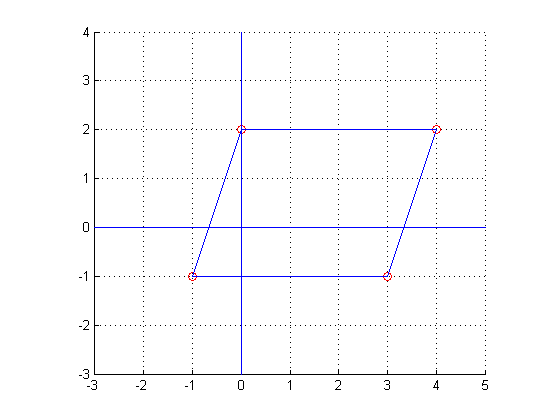
\includegraphics[width=10cm]{para}
%\end{frigure}

\end{frame}

%%%%%%%%%%%%%%%%%%%%%%%%%%%%%%%%%%%%%%%%%%%%%%%%%%%%%%%%%%%%%%%%%%%%%

\begin{frame}

\frametitle{Trapez}

Natanko en od parametrov $p_0, p_1, p_2$ je enak 1. 
Obstaja natanko ena interpolacijska krivulja.

%\begin{itemize}
%\item Če je $p_0 = 1$, je rešitev $\al = \frac{p_1 + 1}{p_1 - 1} = \frac{p_2 - 1}{p_2 + 1}$,
%\item Če je $p_1 = 1$, je rešitev $\al = \frac{p_0 + 1}{2}$,
%\item Če je $p_2 = 1$, je rešitev $\al = \frac{2}{p_0 + 1} = \frac{2}{1-p_2}$.
%\end{itemize}

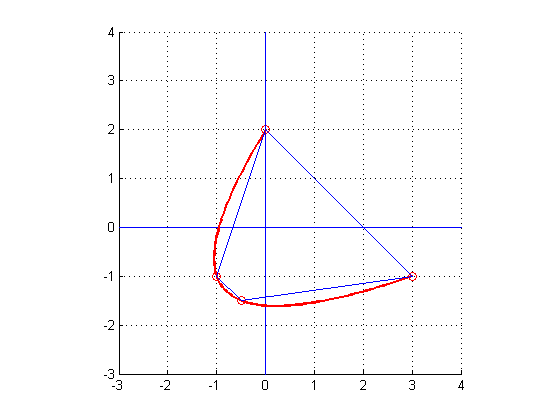
\includegraphics[width=10cm]{trap}

%\begin{wrapfigure}{r}{7cm} %this figure will be at the right
%    \centering
%    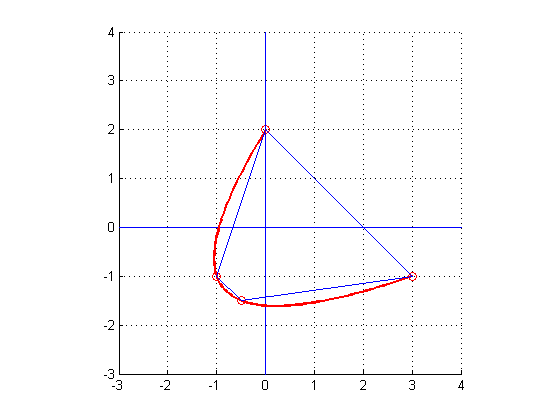
\includegraphics[width=8cm]{trap}
%\end{wrapfigure}
%%Vrednost $\al$  izračunamo tako 

\end{frame}

%%%%%%%%%%%%%%%%%%%%%%%%%%%%%%%%%%%%%%%%%%%%%%%%%%%%%%%%%%%%%%%%%%%%%

\begin{frame}

\frametitle{Konveksen lik}

Noben od parametrov $p_0, p_1, p_2$ ni enak 1, produkt $p_0 p_1 p_2$ je negativen. Točke lahko interpoliramo z dvema paraboličnima krivuljama.

%\begin{figure}[h]
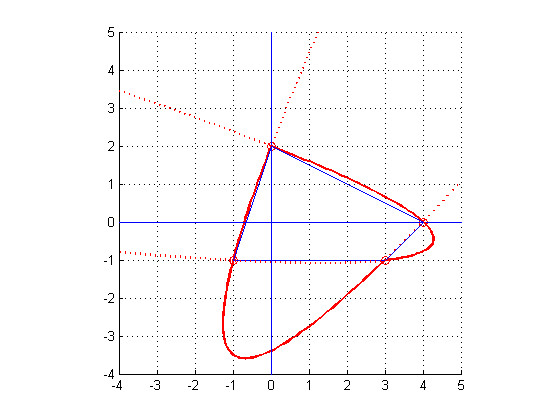
\includegraphics[width=9cm]{konv}
%\end{frigure}

\end{frame}

%%%%%%%%%%%%%%%%%%%%%%%%%%%%%%%%%%%%%%%%%%%%%%%%%%%%%%%%%%%%%%%%%%%%%

\begin{frame}

\frametitle{Konkaven lik}

Noben od parametrov $p_0, p_1, p_2$ ni enak 1,  produkt $p_0 p_1 p_2$ je pozitiven. Točk ne moremo interpolirati s parabolično krivuljo.

%\begin{figure}[h]
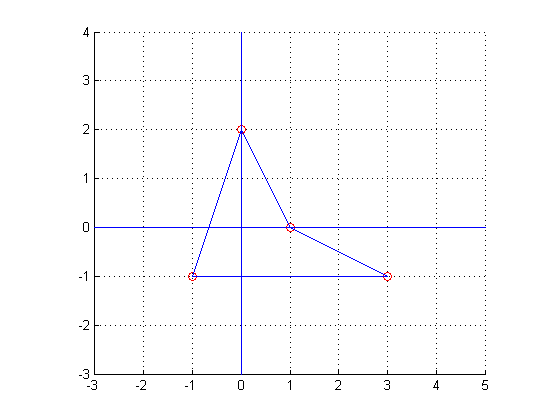
\includegraphics[width=10cm]{konk}
%\end{frigure}

\end{frame}

%%%%%%%%%%%%%%%%%%%%%%%%%%%%%%%%%%%%%%%%%%%%%%%%%%%%%%%%%%%%%%%%%%%%%


\end{document}